% Options for packages loaded elsewhere
\PassOptionsToPackage{unicode}{hyperref}
\PassOptionsToPackage{hyphens}{url}
\PassOptionsToPackage{dvipsnames,svgnames,x11names}{xcolor}
%
\documentclass[
  singlecolumn]{report}

\usepackage{amsmath,amssymb}
\usepackage{iftex}
\ifPDFTeX
  \usepackage[T1]{fontenc}
  \usepackage[utf8]{inputenc}
  \usepackage{textcomp} % provide euro and other symbols
\else % if luatex or xetex
  \usepackage{unicode-math}
  \defaultfontfeatures{Scale=MatchLowercase}
  \defaultfontfeatures[\rmfamily]{Ligatures=TeX,Scale=1}
\fi
\usepackage[]{libertinus}
\ifPDFTeX\else  
    % xetex/luatex font selection
\fi
% Use upquote if available, for straight quotes in verbatim environments
\IfFileExists{upquote.sty}{\usepackage{upquote}}{}
\IfFileExists{microtype.sty}{% use microtype if available
  \usepackage[]{microtype}
  \UseMicrotypeSet[protrusion]{basicmath} % disable protrusion for tt fonts
}{}
\makeatletter
\@ifundefined{KOMAClassName}{% if non-KOMA class
  \IfFileExists{parskip.sty}{%
    \usepackage{parskip}
  }{% else
    \setlength{\parindent}{0pt}
    \setlength{\parskip}{6pt plus 2pt minus 1pt}}
}{% if KOMA class
  \KOMAoptions{parskip=half}}
\makeatother
\usepackage{xcolor}
\usepackage[top=30mm,left=20mm,heightrounded]{geometry}
\setlength{\emergencystretch}{3em} % prevent overfull lines
\setcounter{secnumdepth}{-\maxdimen} % remove section numbering
% Make \paragraph and \subparagraph free-standing
\ifx\paragraph\undefined\else
  \let\oldparagraph\paragraph
  \renewcommand{\paragraph}[1]{\oldparagraph{#1}\mbox{}}
\fi
\ifx\subparagraph\undefined\else
  \let\oldsubparagraph\subparagraph
  \renewcommand{\subparagraph}[1]{\oldsubparagraph{#1}\mbox{}}
\fi


\providecommand{\tightlist}{%
  \setlength{\itemsep}{0pt}\setlength{\parskip}{0pt}}\usepackage{longtable,booktabs,array}
\usepackage{calc} % for calculating minipage widths
% Correct order of tables after \paragraph or \subparagraph
\usepackage{etoolbox}
\makeatletter
\patchcmd\longtable{\par}{\if@noskipsec\mbox{}\fi\par}{}{}
\makeatother
% Allow footnotes in longtable head/foot
\IfFileExists{footnotehyper.sty}{\usepackage{footnotehyper}}{\usepackage{footnote}}
\makesavenoteenv{longtable}
\usepackage{graphicx}
\makeatletter
\def\maxwidth{\ifdim\Gin@nat@width>\linewidth\linewidth\else\Gin@nat@width\fi}
\def\maxheight{\ifdim\Gin@nat@height>\textheight\textheight\else\Gin@nat@height\fi}
\makeatother
% Scale images if necessary, so that they will not overflow the page
% margins by default, and it is still possible to overwrite the defaults
% using explicit options in \includegraphics[width, height, ...]{}
\setkeys{Gin}{width=\maxwidth,height=\maxheight,keepaspectratio}
% Set default figure placement to htbp
\makeatletter
\def\fps@figure{htbp}
\makeatother

\usepackage{booktabs}
\usepackage{longtable}
\usepackage{array}
\usepackage{multirow}
\usepackage{wrapfig}
\usepackage{float}
\usepackage{colortbl}
\usepackage{pdflscape}
\usepackage{tabu}
\usepackage{threeparttable}
\usepackage{threeparttablex}
\usepackage[normalem]{ulem}
\usepackage{makecell}
\usepackage{xcolor}
\makeatletter
\makeatother
\makeatletter
\makeatother
\makeatletter
\@ifpackageloaded{caption}{}{\usepackage{caption}}
\AtBeginDocument{%
\ifdefined\contentsname
  \renewcommand*\contentsname{Table of contents}
\else
  \newcommand\contentsname{Table of contents}
\fi
\ifdefined\listfigurename
  \renewcommand*\listfigurename{List of Figures}
\else
  \newcommand\listfigurename{List of Figures}
\fi
\ifdefined\listtablename
  \renewcommand*\listtablename{List of Tables}
\else
  \newcommand\listtablename{List of Tables}
\fi
\ifdefined\figurename
  \renewcommand*\figurename{Figure}
\else
  \newcommand\figurename{Figure}
\fi
\ifdefined\tablename
  \renewcommand*\tablename{Table}
\else
  \newcommand\tablename{Table}
\fi
}
\@ifpackageloaded{float}{}{\usepackage{float}}
\floatstyle{ruled}
\@ifundefined{c@chapter}{\newfloat{codelisting}{h}{lop}}{\newfloat{codelisting}{h}{lop}[chapter]}
\floatname{codelisting}{Listing}
\newcommand*\listoflistings{\listof{codelisting}{List of Listings}}
\makeatother
\makeatletter
\@ifpackageloaded{caption}{}{\usepackage{caption}}
\@ifpackageloaded{subcaption}{}{\usepackage{subcaption}}
\makeatother
\makeatletter
\@ifpackageloaded{tcolorbox}{}{\usepackage[skins,breakable]{tcolorbox}}
\makeatother
\makeatletter
\@ifundefined{shadecolor}{\definecolor{shadecolor}{rgb}{.97, .97, .97}}
\makeatother
\makeatletter
\makeatother
\makeatletter
\makeatother
\ifLuaTeX
  \usepackage{selnolig}  % disable illegal ligatures
\fi
\IfFileExists{bookmark.sty}{\usepackage{bookmark}}{\usepackage{hyperref}}
\IfFileExists{xurl.sty}{\usepackage{xurl}}{} % add URL line breaks if available
\urlstyle{same} % disable monospaced font for URLs
\hypersetup{
  pdftitle={Better Causal Diagrammes},
  pdfauthor={Joseph A. Bulbulia},
  colorlinks=true,
  linkcolor={blue},
  filecolor={Maroon},
  citecolor={Blue},
  urlcolor={Blue},
  pdfcreator={LaTeX via pandoc}}

\title{Better Causal Diagrammes}
\author{Joseph A. Bulbulia}
\date{}

\begin{document}
\maketitle
\ifdefined\Shaded\renewenvironment{Shaded}{\begin{tcolorbox}[interior hidden, breakable, sharp corners, enhanced, frame hidden, boxrule=0pt, borderline west={3pt}{0pt}{shadecolor}]}{\end{tcolorbox}}\fi

\listoffigures
\listoftables
\hypertarget{introduction}{%
\section{Introduction}\label{introduction}}

\hypertarget{objective}{%
\subsection{Objective}\label{objective}}

The frequent misconception of equating correlation with causation in
human sciences has given rise to a \textbf{causal crisis} {[}cite{]}.
Despite the potential of causal diagrams to address this predicament,
their practicality is sometimes obscured by confusion and improper
utalisation.

Here, we:

\begin{enumerate}
\def\labelenumi{\arabic{enumi}.}
\item
  develop the connection between this powerful analytical tool and the
  potential outcomes framework, a fundamental component of causal
  inference.
\item
  offer practical guidance for employing causal diagrams to enhance
  causal understanding for questions in the human sciences, to
  accellerate the transition from merely inferring correlations to
  estimating causal relationships.
\item
  emphasise the need for time-series data to address causal questions,
  such that the chronological sequence of events implied by the
  diagramme may identify cause-effect relationships.
\end{enumerate}

We apply the tools to a problem of measurement error in time-series
data.

Our overarching goal is to deliver a comprehensive tutorial that
elucidates the principles of causal inference and showcases the
practical utility of causal diagrams, encouraging a more precise and
informed approach to discerning causality.

\hypertarget{correlation}{%
\subsection{Correlation}\label{correlation}}

Correlation is not, in itself, the problem. We say a relation between an
exposure \(A\) and and outcome \(Y\) is causal if the corration between
\(A\) and \(Y\) is unbiased.

Causal diagrammes, or directed acyclic graphs (DAGS), are qualitative
tools for identifying sources of bias. They are powerful because they
translate a mathematical artiface that underpinns causal inference into
simple, useable images. We may therefore use the images to understand
how we may answer causal questions.

However we must recognise that we never start by answering a causal
question. We start by asking a causal question. Many who utilise causal
graphs fail to appreciate this fact.

\hypertarget{the-potential-outcomes-framework.}{%
\section{The potential outcomes
framework.}\label{the-potential-outcomes-framework.}}

\hypertarget{causal-consistency}{%
\subsection{Causal consistency}\label{causal-consistency}}

\hypertarget{postivity}{%
\subsection{Postivity}\label{postivity}}

\hypertarget{exchangeability}{%
\subsection{Exchangeability}\label{exchangeability}}

\hypertarget{correct-model-specification}{%
\subsection{Correct model
specification}\label{correct-model-specification}}

\hypertarget{the-four-canonical-causal-diagrammes-problems-and-solutions}{%
\section{The Four Canonical Causal Diagrammes: Problems and
Solutions}\label{the-four-canonical-causal-diagrammes-problems-and-solutions}}

\hypertarget{confounding-by-common-cause}{%
\subsection{1. Confounding by Common
Cause}\label{confounding-by-common-cause}}

The problem of confounding by common cause arises when there is an
unmeasured or unaccounted-for variable, denoted as ``L,'' that
influences both the treatment variable, denoted by \(A,\) and the
outcome variable, denoted as \(Y.\) This confounder, \(L\), creates an
association between \(A\) and \(Y\) that is not solely due to the direct
causal effect of \(A\) on \(Y\). Instead, the observed association
between \(A\) and \(Y\) may be partially or entirely driven by the
presence of \(L\), making it difficult to isolate and accurately
estimate the true causal effect of \(A\) on \(Y\).

\begin{figure}

{\centering 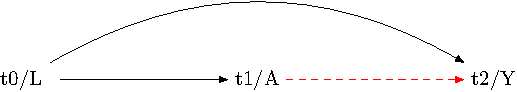
\includegraphics[width=1\textwidth,height=\textheight]{causal-dags_files/figure-pdf/fig-dag-common-cause-1.pdf}

}

\caption{\label{fig-dag-common-cause}Counfounding by common cause.}

\end{figure}

\hypertarget{solution-adjust-for-the-pre-exposure-confounder}{%
\subsection{Solution: adjust for the pre-exposure
confounder}\label{solution-adjust-for-the-pre-exposure-confounder}}

Confounding by common cause can be addressed by adjusting for it. If
\(L\) is measured before the treatment (or exposure) is assigned, we may
adjust for this confounder to account for its influence. Typically we
adjust through through statistical techniques such as stratification,
regression, matching, or inverse probability of treatment weighting.
Sucg adjustment helps to mitigate the bias caused by the confounder,
allowing for a more accurate estimation of the true causal relationship.

\begin{figure}

{\centering 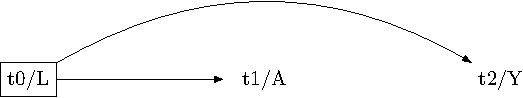
\includegraphics[width=1\textwidth,height=\textheight]{causal-dags_files/figure-pdf/fig-dag-common-cause-solution-1.pdf}

}

\caption{\label{fig-dag-common-cause-solution}Solution: adjust for
pre-exposure confounder.}

\end{figure}

\hypertarget{collider-stratification-conditioning-on-a-common-effect}{%
\subsection{2, collider stratification: conditioning on a common
effect}\label{collider-stratification-conditioning-on-a-common-effect}}

Conditioning on a common effect occures when a variable \(L\) is
affected by both the treatment \(A\) and an outcome \(Y\). Conditioning
on \(L\) creates a spurious association between \(A\) and \(Y\), biasing
the true causal relationship. This occurs because the relationship
between \(A\) and \(Y\) becomes confounded by the common effect \(L\).
The observed association between \(A\) and \(Y\) may be solely driven by
the influence of \(L\).

\begin{figure}

{\centering 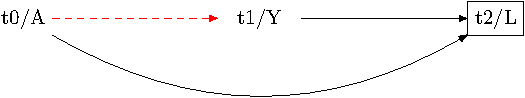
\includegraphics[width=1\textwidth,height=\textheight]{causal-dags_files/figure-pdf/fig-dag-common-effect-1.pdf}

}

\caption{\label{fig-dag-common-effect}Solution: ensure confounder is
measured prior to the exposure.}

\end{figure}

\hypertarget{solution-ensure-all-confounders-are-measured-before-the-exposure}{%
\subsection{Solution: ensure all confounders are measured before the
exposure}\label{solution-ensure-all-confounders-are-measured-before-the-exposure}}

To address the problem of conditioning on a common effect, it is crucial
to ensure that every potential confounder \(L\) that may affect \(A\) is
measured before \(A\). If such temporal order is preserved, \(L\) cannot
be an effect of \(A\), and thus neither of \(Y\). By measuring all
relevant confounders in advance, researchers can minimize bias and
obtain more reliable estimates of the true causal relationship between A
and Y. Note that collider stratification may arise even if \(L\) occurs
before \(A\), when \(L\) does not affect \(A\) or \(Y\). This is called
M-bias. We describe this case below. Note, however, that if \(L\) is not
a common cause of \(A\) and \(Y\), \(L\) should not be included in our
model because it is not a source of confounding.

\begin{figure}

{\centering 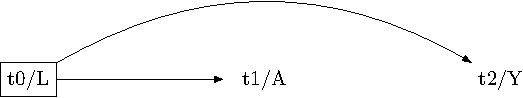
\includegraphics[width=1\textwidth,height=\textheight]{causal-dags_files/figure-pdf/fig-dag-common-effect-solution-1.pdf}

}

\caption{\label{fig-dag-common-effect-solution}Causal graph reveals
bias: solve by stratification}

\end{figure}

\hypertarget{conditioning-on-a-mediator}{%
\subsection{3 Conditioning on a
mediator}\label{conditioning-on-a-mediator}}

Conditioning on a mediator refers to a situation where \(L\) lies on the
causal pathway between the treatment \(A\) and the outcome \(Y\).
Conditioning on \(L\) can lead to biased estimates by blocking or
distort the true causal pathway between \(A\) and \(Y\), obscuring the
total effect of \(A\) on \(Y\). Where \(L\) is a collider between \(A\)
and an unmeasured confouder \(U\), then including \(L\) may increase the
strength of association between \(A\) and \(Y\). We review this second
possibility next. In either case, unless one is interested in mediation
analysis (see below), conditioning on a post-treatment variable is
nearly always a bad idea. {[}JB to discuss the exception{]}

\begin{figure}

{\centering 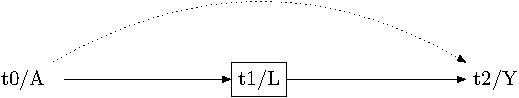
\includegraphics[width=1\textwidth,height=\textheight]{causal-dags_files/figure-pdf/fig-dag-mediator-1.pdf}

}

\caption{\label{fig-dag-mediator}Third problem: conditioning on a
mediator.}

\end{figure}

\hypertarget{solution-ensure-confounders-are-measured-before-the-exposure}{%
\subsection{Solution: ensure confounders are measured before the
exposure}\label{solution-ensure-confounders-are-measured-before-the-exposure}}

To address the problem of mediator bias, when interested in total
effects do not condition on a mediator. This can be done by ensuring
that \(L\) occurs before \(A\) (and \(Y\)). Again we discover the
importance of an explicit temporal ordering for our variables. Although
note, if \(L\) is associated with \(Y\) but is not associated with \(A\)
conditioning on \(L\) will improve the efficiency of the causal effect
estimate of \(A\) on \(Y\). However, if \(A\) might affect \(L\), then
\(L\) might be a mediator, and including \(L\) risks bias. As with some
much in causal estimation, we must understand the context.

\begin{figure}

{\centering 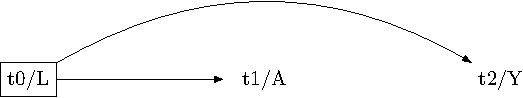
\includegraphics[width=1\textwidth,height=\textheight]{causal-dags_files/figure-pdf/fig-dag-mediator-solution-1.pdf}

}

\caption{\label{fig-dag-mediator-solution}Do not condition on a
mediator}

\end{figure}

\hypertarget{conditioning-on-a-descendant}{%
\subsection{4. conditioning on a
descendant}\label{conditioning-on-a-descendant}}

Say \(A\) is a cause of \(A*\). There is a theorem that proves that when
we condition on \(A*\) we partially condition on \(A\).

There are both negative and positive implications of this theorem for
causal estimation in real-world scenarios.

First the negative. Suppose there is a confounder \(L\) that is caused
by an unobserved variable \(U\), and is affected by the treatment \(A\).
Suppose further that \(U\) causes the outcome \(Y\). In this scenario,
as described in Figure~\ref{fig-dag-descendent}, conditioning on \(L\),
which is a descendant of \(A\) and \(U\), can lead to a spurious
association between \(A\) and \(Y\) through the path
\(A \to L \to U \to Y\).

\begin{figure}

{\centering 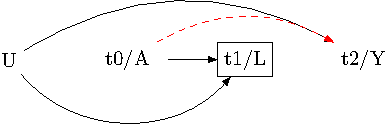
\includegraphics[width=1\textwidth,height=\textheight]{causal-dags_files/figure-pdf/fig-dag-descendent-1.pdf}

}

\caption{\label{fig-dag-descendent}Conditioning on a descendant}

\end{figure}

\hypertarget{solution-ensure-that-counfounders-are-measured-before-the-exposure}{%
\subsection{Solution: ensure that counfounders are measured before the
exposure}\label{solution-ensure-that-counfounders-are-measured-before-the-exposure}}

Ensuring the confounder (L) is measured before the exposure (A) has two
beneficial properties. Firstly, if \(L\) is a confounder, that is, if
\(L\) is a variable which if we fail to condition on it will bias the
association between treatment and outcome, the strategy of including
only pre-treatment indicators of \(L\) will eliminate collider bias.
Secondly, there is the positive side to the theorem that conditioning on
a descendent is equivalent to partially conditioning on its parent: if
an unmeasured confounder is associated with both \(A\), \(Y\), and
\(L\), then adjusting for \(L\) helps to reduce confounding caused by
the unmeasured confounder. By obtaining measure of \(L\) that occur
before \(A\), such advantages can be achieved, allowing for more
accurate estimation for the causal effect of \(A\) on \(Y\). We use the
convention of a blue dotted arrow to indicate that the association
between \(A\) and \(Y\) may still be biased, but that bias is reduced by
inluding \(L\)

\begin{figure}

{\centering 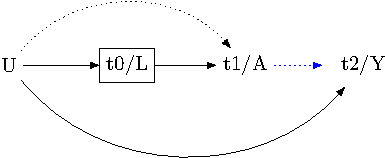
\includegraphics[width=1\textwidth,height=\textheight]{causal-dags_files/figure-pdf/fig-dag-descendent-solution-1.pdf}

}

\caption{\label{fig-dag-descendent-solution}Solution: conditioning on a
descendent is part of the solution, not the problem, when baseline
confounders are measured before the exposure.}

\end{figure}

\textbf{This ends the examples of cannoical casual diagrammes}

\hypertarget{summary}{%
\subsection{Summary}\label{summary}}

\hypertarget{common-cause-of-exposure-and-outcome.}{%
\section{Common cause of exposure and
outcome.}\label{common-cause-of-exposure-and-outcome.}}

\begin{figure}

{\centering 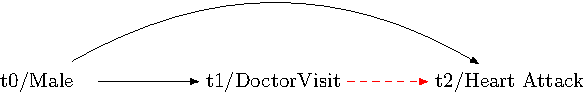
\includegraphics[width=1\textwidth,height=\textheight]{causal-dags_files/figure-pdf/fig-dag-1-1.pdf}

}

\caption{\label{fig-dag-1}Common cause of exposure and outcome: example}

\end{figure}

\hypertarget{solution-adjust-for-confounder}{%
\subsection{Solution: Adjust for
Confounder}\label{solution-adjust-for-confounder}}

\begin{figure}

{\centering 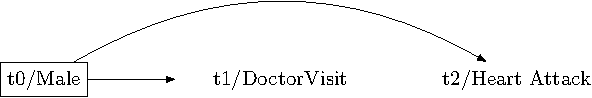
\includegraphics[width=1\textwidth,height=\textheight]{causal-dags_files/figure-pdf/fig-dag-2-1.pdf}

}

\caption{\label{fig-dag-2}Solution to this problem.}

\end{figure}

\hypertarget{bias-exposure-at-baseline-is-a-common-cause-of-the-exposure-at-t1-and-outcome-at-t2}{%
\subsection{Bias: exposure at baseline is a common cause of the exposure
at t1 and outcome at
t2}\label{bias-exposure-at-baseline-is-a-common-cause-of-the-exposure-at-t1-and-outcome-at-t2}}

\begin{figure}

{\centering 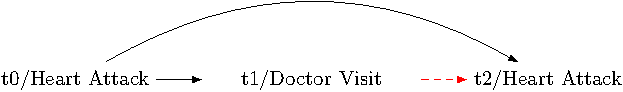
\includegraphics[width=1\textwidth,height=\textheight]{causal-dags_files/figure-pdf/fig-dag-3-1.pdf}

}

\caption{\label{fig-dag-3}Causal graph reveals bias from pre-exosure
indicator}

\end{figure}

\hypertarget{solution-adjust-for-confounder-at-baseline}{%
\subsection{Solution: adjust for confounder at
baseline}\label{solution-adjust-for-confounder-at-baseline}}

\begin{figure}

{\centering 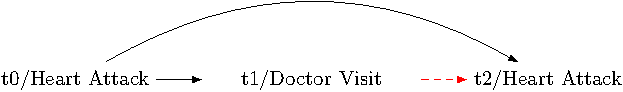
\includegraphics[width=1\textwidth,height=\textheight]{causal-dags_files/figure-pdf/fig-dag-4-1.pdf}

}

\caption{\label{fig-dag-4}Solution to this problem}

\end{figure}

\hypertarget{a-more-thorough-confounding-control}{%
\subsection{A more thorough confounding
control}\label{a-more-thorough-confounding-control}}

\begin{figure}

{\centering 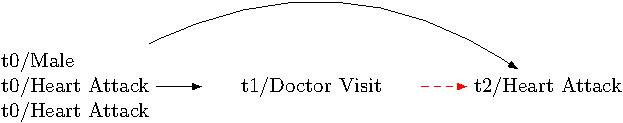
\includegraphics[width=1\textwidth,height=\textheight]{causal-dags_files/figure-pdf/fig-dag-5-1.pdf}

}

\caption{\label{fig-dag-5}Causal graph:more general panel design}

\end{figure}

\hypertarget{generic-3-wave-panel-design-vanderweeele-2020}{%
\subsection{Generic 3-wave panel design (VanderWeeele
2020)}\label{generic-3-wave-panel-design-vanderweeele-2020}}

\begin{figure}

{\centering 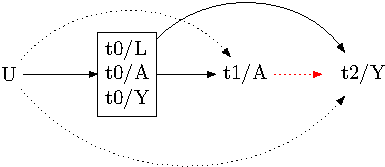
\includegraphics[width=1\textwidth,height=\textheight]{causal-dags_files/figure-pdf/fig-dag-6-1.pdf}

}

\caption{\label{fig-dag-6}Causal graph: three-wave panel design}

\end{figure}

\hypertarget{selection-bias-there-are-several-types}{%
\subsection{Selection bias: there are several
types}\label{selection-bias-there-are-several-types}}

\hypertarget{unmeasured-confounder-affects-selection-and-the-outcome}{%
\subsubsection{Unmeasured confounder affects selection and the
outcome}\label{unmeasured-confounder-affects-selection-and-the-outcome}}

\begin{figure}

{\centering 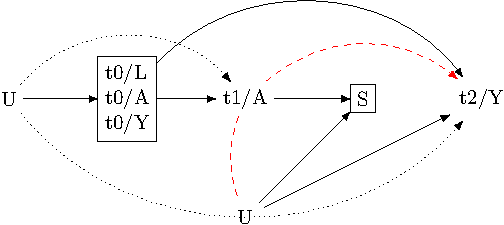
\includegraphics[width=1\textwidth,height=\textheight]{causal-dags_files/figure-pdf/fig-dag-8-1.pdf}

}

\caption{\label{fig-dag-8}Causal graph: three-wave panel design with
selection bias}

\end{figure}

\hypertarget{unmeasured-confounder-affects-a-measured-confounder-of-selection-and-the-outcome-and-there-are-unmeasured-confourders-that-affect-the-measured-confounder}{%
\subsubsection{Unmeasured confounder affects a measured confounder of
selection and the outcome, and there are unmeasured confourders that
affect the measured
confounder}\label{unmeasured-confounder-affects-a-measured-confounder-of-selection-and-the-outcome-and-there-are-unmeasured-confourders-that-affect-the-measured-confounder}}

\begin{figure}

{\centering 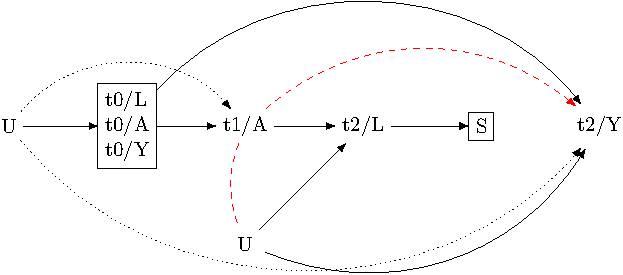
\includegraphics[width=1\textwidth,height=\textheight]{causal-dags_files/figure-pdf/fig-dag-8-2-1.pdf}

}

\caption{\label{fig-dag-8-2}Causal graph: three-wave panel design with
selection bias: example 2}

\end{figure}

\hypertarget{unmeasured-confounder-affects-slection-into-the-study-and-also-attrition}{%
\subsubsection{Unmeasured confounder affects slection into the study and
also
attrition}\label{unmeasured-confounder-affects-slection-into-the-study-and-also-attrition}}

\begin{figure}

{\centering 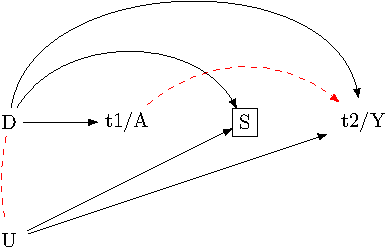
\includegraphics[width=1\textwidth,height=\textheight]{causal-dags_files/figure-pdf/fig-dag-8-4-1.pdf}

}

\caption{\label{fig-dag-8-4}Causal graph: three-wave panel design with
selection bias: selection into the study (D) affects attrition}

\end{figure}

\hypertarget{outcome-and-exposure-affect-attrition}{%
\subsubsection{Outcome and exposure affect
attrition}\label{outcome-and-exposure-affect-attrition}}

\begin{figure}

{\centering 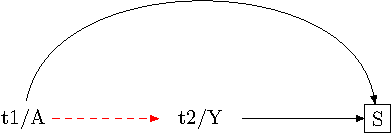
\includegraphics[width=1\textwidth,height=\textheight]{causal-dags_files/figure-pdf/fig-dag-8-5-1.pdf}

}

\caption{\label{fig-dag-8-5}Causal graph:outcome and exposure affect
attrition (Y measured with directed measurement error)}

\end{figure}

\hypertarget{outcome-and-exposure-affect-attrition-we-may-approach-this-problem-as-one-of-directed-measurement-error.}{%
\subsubsection{Outcome and exposure affect attrition: we may approach
this problem as one of directed measurement
error.}\label{outcome-and-exposure-affect-attrition-we-may-approach-this-problem-as-one-of-directed-measurement-error.}}

\begin{figure}

{\centering 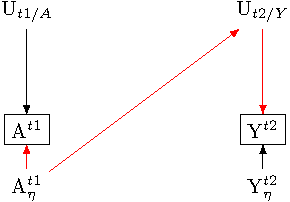
\includegraphics[width=1\textwidth,height=\textheight]{causal-dags_files/figure-pdf/fig-directed-measurement-error-1.pdf}

}

\caption{\label{fig-directed-measurement-error}TBA}

\end{figure}

\hypertarget{important-causal-diagrammes}{%
\section{Important Causal
Diagrammes}\label{important-causal-diagrammes}}

\hypertarget{how-do-we-draw-interactions}{%
\section{How do we draw
interactions?}\label{how-do-we-draw-interactions}}

\hypertarget{common-cause-of-exposure-and-outcome.-1}{%
\section{Common cause of exposure and
outcome.}\label{common-cause-of-exposure-and-outcome.-1}}

\begin{figure}

{\centering 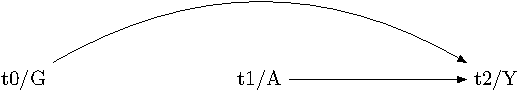
\includegraphics[width=1\textwidth,height=\textheight]{causal-dags_files/figure-pdf/fig-dag-effect-modfication-1.pdf}

}

\caption{\label{fig-dag-effect-modfication}A simple graph for
effect-modification.}

\end{figure}

\hypertarget{another-graph-for-interaction}{%
\subsection{Another graph for
interaction}\label{another-graph-for-interaction}}

\begin{figure}

{\centering 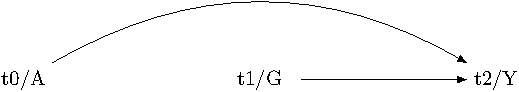
\includegraphics[width=1\textwidth,height=\textheight]{causal-dags_files/figure-pdf/fig-dag-effect-modfication-2-1.pdf}

}

\caption{\label{fig-dag-effect-modfication-2}A simple graph for
effect-modification.}

\end{figure}

\hypertarget{m-bias}{%
\subsection{M-Bias}\label{m-bias}}

\begin{figure}

{\centering 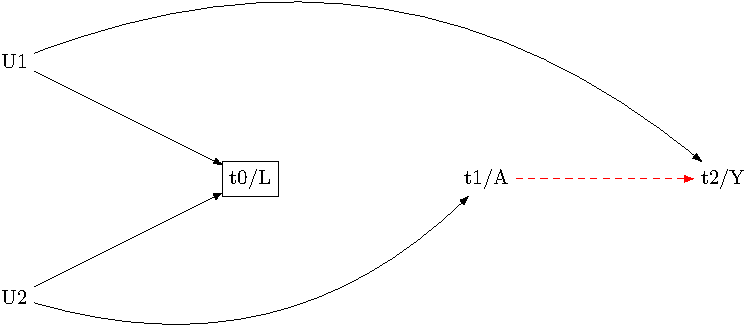
\includegraphics[width=1\textwidth,height=\textheight]{causal-dags_files/figure-pdf/fig-m-bias-1.pdf}

}

\caption{\label{fig-m-bias}M-bias: confounding control by including
previous measures of the outcome}

\end{figure}

\hypertarget{what-if-mediation-is-of-interest}{%
\subsection{What if mediation is of
interest?}\label{what-if-mediation-is-of-interest}}

Consider the assumptions required for mediation analysis:

\begin{enumerate}
\def\labelenumi{\arabic{enumi}.}
\tightlist
\item
  No unmeasured exposure-outcome confounders given \(L\)
\end{enumerate}

\[Y^{am}\coprod A|L\] 2. No unmeasured meadiator-outcome confounders
given \(L\)

\[Y^{am}\coprod M|L\]

\begin{enumerate}
\def\labelenumi{\arabic{enumi}.}
\setcounter{enumi}{2}
\tightlist
\item
  No unmeasured exposure-mediator confounders given \(L\)
\end{enumerate}

\[M^{a}\coprod A|L\]

\begin{enumerate}
\def\labelenumi{\arabic{enumi}.}
\setcounter{enumi}{3}
\tightlist
\item
  No mediator-outcome confounder affected by the exposure (no red arrow)
\end{enumerate}

\[Y^{am}\coprod M^{a*}|L\]

\begin{figure}

{\centering 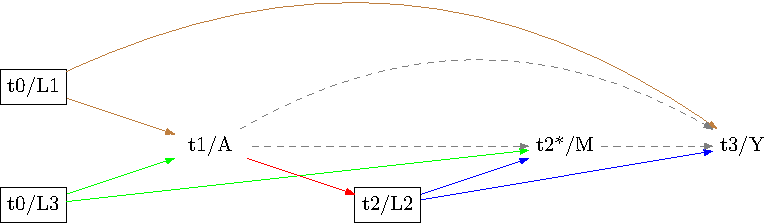
\includegraphics[width=1\textwidth,height=\textheight]{causal-dags_files/figure-pdf/fig-dag-mediation-assuptions-1.pdf}

}

\caption{\label{fig-dag-mediation-assuptions}Assumptions for mediation
analysis}

\end{figure}

\hypertarget{confounder-treatment-feedback}{%
\subsection{Confounder-Treatment
Feedback}\label{confounder-treatment-feedback}}

\begin{figure}

{\centering 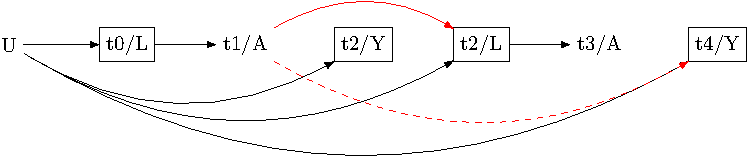
\includegraphics[width=1\textwidth,height=\textheight]{causal-dags_files/figure-pdf/fig-dag-9-1.pdf}

}

\caption{\label{fig-dag-9}Confounder Treatement Feedback}

\end{figure}

\hypertarget{multiple-versions-of-treatment}{%
\section{Multiple Versions of
Treatment}\label{multiple-versions-of-treatment}}

\begin{figure}

{\centering 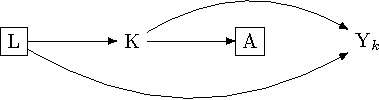
\includegraphics[width=1\textwidth,height=\textheight]{causal-dags_files/figure-pdf/fig_dag_multiple_version_treatment_dag-1.pdf}

}

\caption{Multiple Versions of treatment. Heae, A is regarded to bbe a
coarseneed version of K}

\end{figure}

\hypertarget{does-the-multiple-versions-of-treatments-approach-save-us}{%
\section{Does the Multiple Versions of Treatments Approach Save
Us?}\label{does-the-multiple-versions-of-treatments-approach-save-us}}

Measurement error remeains a problem if errors are either directed or
dependent (correlated) or both. (See: measurement link.)

\begin{figure}

{\centering 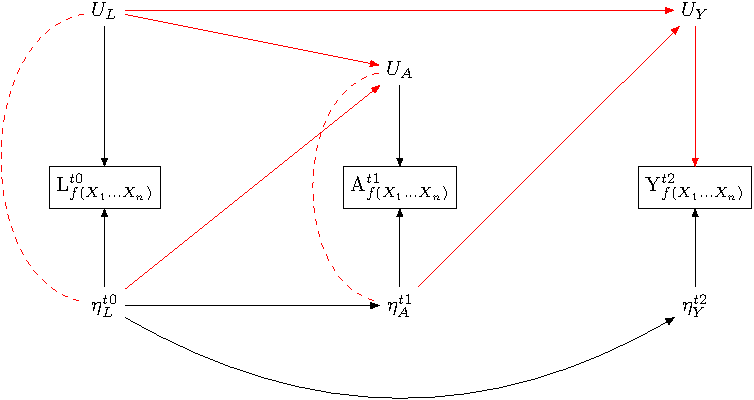
\includegraphics[width=1\textwidth,height=\textheight]{causal-dags_files/figure-pdf/fig-dag-dep-udir-effect-confounders-3wave-1.pdf}

}

\caption{\label{fig-dag-dep-udir-effect-confounders-3wave}Measurement
error opens a pathway to confounding if either there are correlated
errors, or a directed effect of the exposure on the errors of measured
outcome.}

\end{figure}

\hypertarget{add-graph-on-when-we-might-want-to-condition-on-a-post-treatment-indicator}{%
\section{Add Graph on when we might want to condition on a post
treatment
indicator}\label{add-graph-on-when-we-might-want-to-condition-on-a-post-treatment-indicator}}

\hypertarget{stray-points-to-address}{%
\section{Stray points to address}\label{stray-points-to-address}}

\begin{enumerate}
\def\labelenumi{\arabic{enumi}.}
\tightlist
\item
  Structural equation models are not causal diagrammes
\item
  Causal diagrammes are non-parametric
\item
  Causal diagrammes represent interactions A -- \textgreater{} Y
  \textless--- B (two arrows into the outcome)
\item
  We may distinguish between effect modification and interaction.
\end{enumerate}



\end{document}
